\section{Methods}

 
\subsection{Modulated Raman Coupling}

Order of ideas here:
Explain how we get SOC, how we modulate it.
Explain pulsing procedure.
Explain effective mass measurement. 




%A spin-orbit coupled spin one system in the presence of a bias magnetic field is described by the Hamiltonian. (This line is awful but I will keep it for now)

We consider a spin one system in a uniform magnetic field  $B\mathbf{e}_z$ that Zeeman splits the energy levels by $\omega_Z/2\pi=g_f\mu_BB = 12 MHz$. A quadratic Zeeman shift $\epsilon$ breaks the $m_F=\pm1\leftrightarrow m_F=0$ degeneracy. We generate spin-orbit coupling between the magnetic sub levels with a pair of intersecting, cross-polarized Raman beams, with wavelength $\lambda=790.33 nm$ propagating along $\mathbf{e}_x+\mathbf{y}$ and $\mathbf{e}_x-\mathbf{e}_y$ as shown in Fig 1a. The system can be fully described by the Hamiltonian

Here I need to introduce delta and frequency differences. 

\begin{align}
	\begin{split}
		\hat{H} = &\frac{\hbar^2\hat{k}^2}{2m} + \alpha_0\hat{k}\hat{F}_z +4E_L\mathbb{I} + \frac{\Omega_R}{2}\hat{F}_x\\
		& +(\epsilon+4E_L)(\hat{F}_z^2-\mathbb{I}) +\Delta_0\hat{F}_z, 
		\label{Eq:SOCone}
	\end{split}]
\end{align}	


where we have introduced the natural units of our system: the single photon recoil momentum $k_L=\frac{2\pi}{\lambda_R}\sin(\theta/2)$ and its associated recoil energy $E_L=\frac{\hbar^2k_L^2}{2m}$, determined by the wavelength and geometry of the Raman field. We have additionally introduced the spin-orbit coupling strength $\alpha_0=\frac{\hbar^2k_L}{m}$ and the Raman coupling strength $\Omega_R$ which is proportional to the field intensity. 

Previous studies have shown that driven systems such as cold atoms in time dependent optical fields[karina, optical lattices, germany group] exhibit effective coupling terms in the Hamiltonian that arise from averaging the dynamics of the system. Here we will show that we can get tunable spin-orbit coupling using a multiple frequency Raman field which is equivalent to periodically modulating the Raman coupling strength.

We choose t
With the addition of these multiple frequency couplings, the Hamiltonian in Eq.\ref{Eq:SOCone} remains unchanged, except for the coupling strength that takes the form $	\Omega_R(t)=\Omega_0 + \Omega\cos(\delta\omega t)$. In order to describe the full quasi-energy spectrum If the driving frequency is chosen so that  $\delta\omega \gg \epsilon$ and $\delta\omega \gg 4E_L$ the effective Hamiltonian retains the form of \ref{Eq:SOCone} with renormalized coefficients and quadratic Zeeman shift, and an additional term that explicitly couples the $m_f=-1$ and $m_f=+1$ states:

In order to describe this time periodic system we can find the quasi-energies using Floquet theory
change here
, or we can find an effective Hamiltonian applying an appropriate time dependent rotation and averaging out fast oscillating terms.


\begin{align}
	\begin{split}
		\hat{H} = &\frac{\hbar^2\hat{k}^2}{2m} + \alpha\hat{k}\hat{F}_z +4E_L\mathbb{I} + \frac{\Omega_0}{2}\hat{F}_x \\
		&+ \frac{\tilde{\Omega}}{2}\hat{F}_{xz} +(\tilde{\epsilon}+4E_L)(\hat{F}_z^2-\mathbb{I}) +\tilde{\Delta}\hat{F}_z, 
		\label{Eq:SOCeff}
	\end{split}
\end{align}	
%
with $\alpha= J_0(\Omega/2\delta\omega)\alpha_0$, $\tilde{\Omega}=1/4(\epsilon+4E_L) (J_0(\Omega/\delta\omega)-1)$, $\Delta=J_0(\Omega/2\delta\omega)\Delta_0$, and $\tilde{\epsilon}= 1/4(4E_L-\epsilon) - 
1/4(4E_L + 3 \epsilon) J_0( \Omega/\delta\omega)$


There are two limiting cases of this effective Hamiltonian \ref{Eq:SOCeff} which will be of interest: (1) for large quadratic Zeeman shift the system can be described as an effective spin $1/2$ (cite Lindsay) system where the spin orbit coupling strength and the Raman coupling can be independently tuned and (2) for small quadratic Zeeman shift we can tune the $m_f=+1\leftrightarrow m_f=-1$ and $m_f=0\leftrightarrow m_f=\pm 1$ coupling strength as well as the spin-orbit coupling strength and the quadratic Zeeman shift, which with the addition of an optical lattice can lead to  measurements of Hofstadter butterfly spectrum(cite synthetic dimensions). In this work we will only focus in the first case. 


In the high field regime, when $\epsilon > 4E_R$, the $m_f=-1\leftrightarrow m_f=0$ and $m_f=0 \leftrightarrow m_f=+1$ transition cannot be resonantly addressed with the same frequency. By adiabatically eliminating the $m_f=0$ state we can describe the system in terms of an effective spin $1/2$  with an effective Hamiltonian

\begin{align}
	\begin{split}
		\hat{H}_{eff} = & \frac{\hbar^2}{2m}(\hat{k}+2\kr\hat{\sigma}_z)^2 + \frac{\hbar\Omega'}{2}\hat{\sigma}_x  +\Delta\hat{\sigma}_z  
	\label{Eq:SOChalf}
	\end{split}
\end{align}	
 
where we have defined an effective coupling between the $m_f=-1$ and $m_f=+1$ states $\Omega'=\tilde{\Omega}+\hbar\Omega_0^2/2(\tilde{\epsilon})$. 


Fig1b shows the hight field dispersion relation, both for the modulated and unmodulated cases (here goes an image of bands). The minima, originally locted at $\pm2 k_L$, are shifted and the size of the spin-orbit gap is changed for different choices of $\Omega_0$, $\Omega$, and $\delta\omega$.  

\begin{figure}
	\begin{center}
		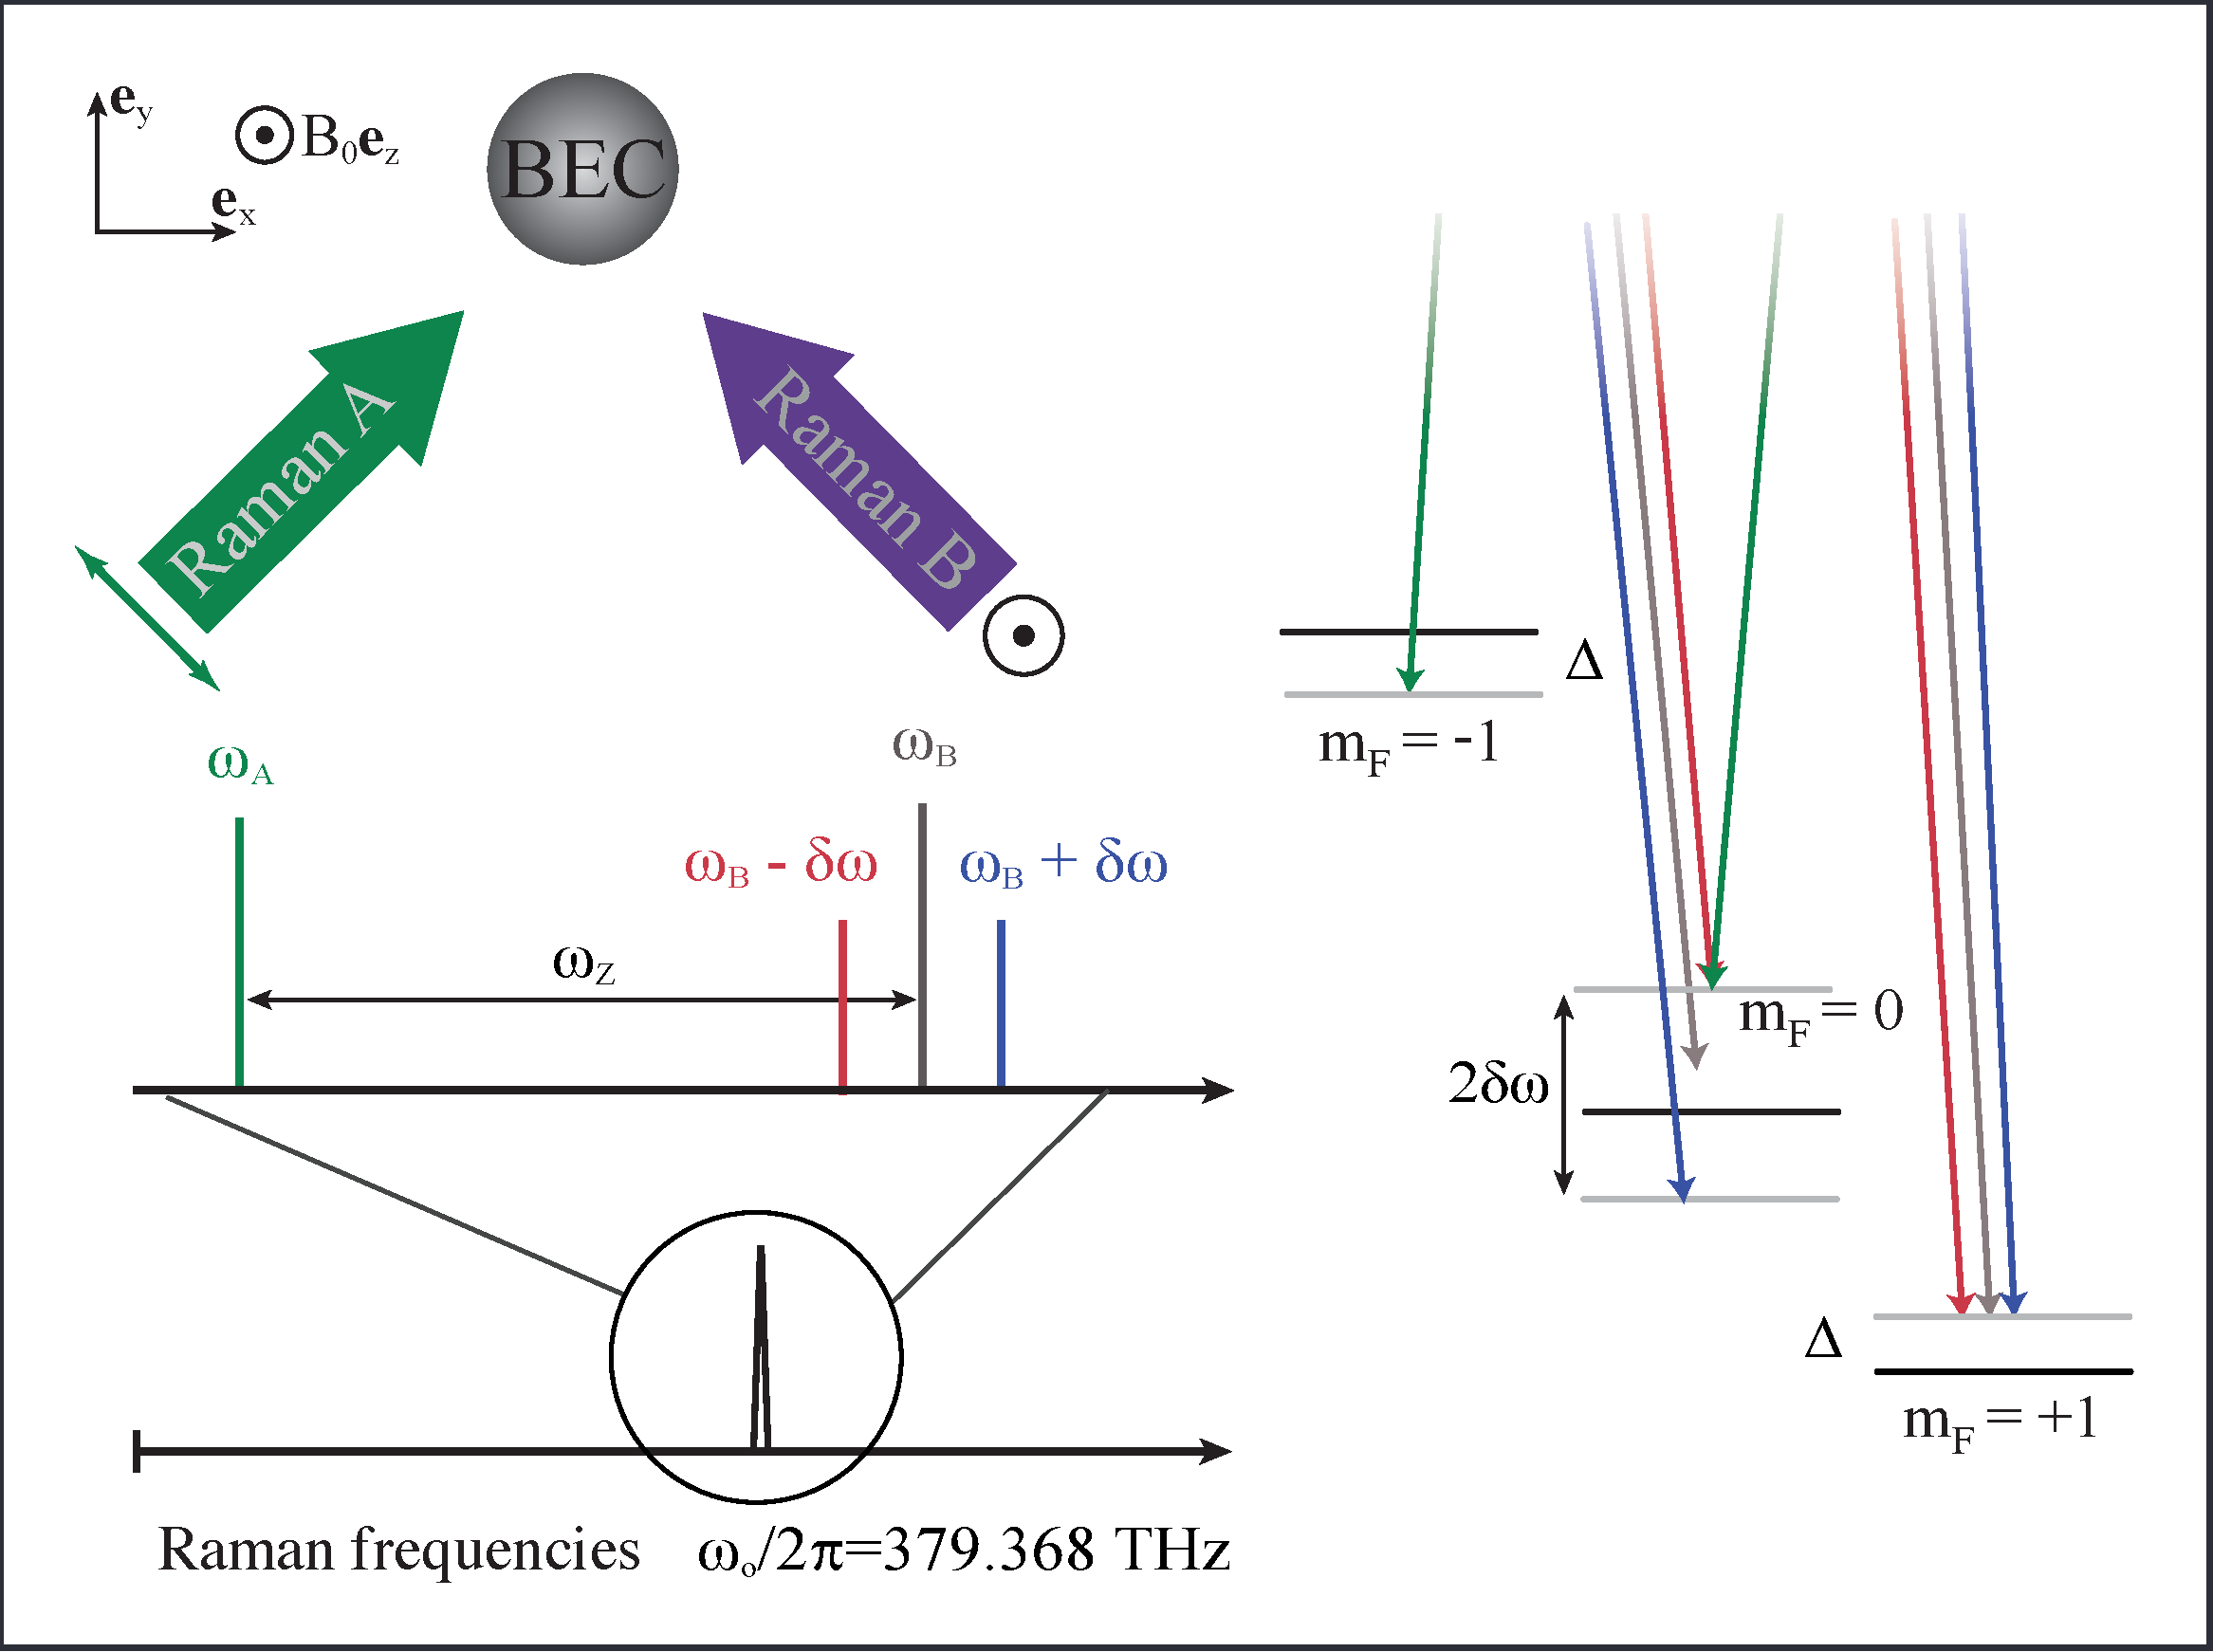
\includegraphics[width=90mm]{\documentpath/laserfreqsv4}
		\caption{{\bf Experimental setup}
		A pair of Raman laser bla bla}
		\label{Fig:Setup}
	\end{center}
\end{figure}




\subsection{Fourier Spectroscopy}		


Think transfer functions and spectroscopy. Spectroscopy is a vertical cut, it looks at response of the system when driven with frequencies within the Fourier limited bandwith of the pulse. 


In order to explicitly measure the modified energy-momentum dispersion relation, we will use a Fourier based spectroscopy technique, which relies on the time evolution of an atomic state after a dressing field is suddenly turned on, and the initially bare states become superpositions of dressed states undergoing Rabi oscillations in time  with spectral components related to the relative energies of the dressed states. 

%as well as for the future measurement of the Hofstadter Butterfly spectrum%


For the case of a spin-orbit coupled atomic system, the dressed state energies are explicitly dependent on both the particle's spin and momentum. Therefore, in order to fully characterize the energy-momentum dispersion we must prepare an atomic state at a given spin and momentum $\ket{k_i,m_{f_i}}$, pulse on the Raman field, and measure the time evolution.  

In practice it may not be as straightforward to reliably prepare an arbitrary momentum state. The measurement however can be simplified by noticing that a non-moving atom cloud in the laboratory reference frame dressed by a field with non-zero detuning is equivalent to a moving cloud with a resonant field in a suitable moving reference frame. This can be explicitly seen in the Hamiltonian \ref{Eq:SOCone} where the detuning term $\delta/Er$  and the momentum term $4 k/k_R$ have the same effect in the relative energies. There is an additional Doppler shift associated with the transformation between reference frames, which gets canceled when we look at the energy differences. Therefore, for the purpose of our experiments, momentum and detuning are equivalent up to a numerical pre factor. 

The method described above only allows us to measure relative energies and we must add a known energy reference if we want to recover the dispersion relation. We can do so by measuring the effective mass $m^{\star} = \hbar^2[\frac{d^2E(k_x)}{dk_x}]^{-1}$ of the nearly quadratic lowest branch of the dispersion, and then shifting the measured frequencies accordingly. 

 Here an image of dispersion, time evolution, FFT, spectrum of energy differences and reconstructed spectrum.

In order to maximize our signal to noise ratio (SNR) and minimize the required number of data points we use some fancy algorithm that I'm still not sure which one will work best. We also choose the spacing and the total number of pulses for each spectra so that the bandwith and resolution of the Fourier transform allow us to resolve the frequencies of interest. 

%The frequencies were extracted using the Lasso algorithm,which given $n$ data points $y$ and $p$ basis functions $x$, seeks to minimize the quantity

%\begin{align}
%\sum_{i=1}^{n}(y_i-\sum_{j}x_{ij}\beta_j)^2+\lambda\sum_{j=1}^{p}\lvert\beta\rvert
%\end{align}

%which is equivalent to a least square fit with a constraint on the L1 norm of the fit coefficients.Here we used the real part of the Fourier basis as our basis functions and the constraint constraint helped to reduce the spectral noise and allowed us to identify the main frequencies of the problem more easily.
%(Tibshirani, 1995)


\subsection{Experimental sequence}


 We start our experimental sequence with a Rb$^{87}$ Bose-Einstein condensate (BEC) with $N\approx 4\times 10^4$ atoms in the $\ket{F=1,m_F=0}$ state, confined in a $1064\nm$ crossed optical dipole trap, with trapping frequencies $(\omega_x,\omega_y,\omega_z)=2\pi(42(3),34(2),133(3))\ \Hz$. We break the degeneracy between the $m_F$ magnetic sub-levels by applying a $17.0556$ G bias field along the z axis, which produces a Zeeman splitting of $12 \ \MHz$ and a quadratic Zeeman shift that lowers the energy of the $\ket{F=1,m_F=0}$ state  by $20.9851$ kHz. 
We use a microwave pulsing protocol (see Supplementary Information) to monitor the bias field and lock it to the desired value. Once the bias field is locked, the sequence we used to study the time evolution of our spin-orbit coupled system was morally the same for all the data we present. For the single frequency case we choose a Raman coupling strength and set the detuning by changing the frequency of our Raman lasers away from four-photon resonance. For the multiple frequency case, when the detuning is set to zero, both $\omega_0$ and $\frac{\omega_+ + \omega_-}{2}$ are at four photon resonance. Otherwise we detune the frequency of $\omega_0$ and $\frac{\omega_+ +\omega_-}{2}$ by the same amount. We suddenly turn on the lasers, let the system evolve for a time $t$, snap off the lasers and let the atoms fall for a $21$ ms time of flight (TOF) time before we image them using resonant absorption imaging. Our images 
reveal the atoms spin and momentum distribution, from which we can extract the full dynamics of the system.


We measure the atom's effective mass by inducing dipole oscillations in our BECs along $\mathbf{e}_x$ and comparing the frequency of oscillation for the bare and dressed atoms case.  We prepare our system in $\ket{F=1,m_F=0}$ and adiabatically turn on the Raman in $xx$ ms while also ramping the detuning to a non-zero value, around $0.5\Er$. This detuning gives a small shift in the energy-momentum minima which causes a small displacement of our BECs. We then suddenly bring the frequency back to resonance (for the dressed state measurement) or turn off the Raman (for the bare state measurement), which excites the dipole mode of our optical dipole trap. We can extract the effective mass from the ratio $m^{\star}/m=\omega^{\star}/\omega$




